\documentclass[12pt,a4paper]{report}

% --- Core packages ---
\usepackage{graphicx}
\usepackage{float}
\usepackage{url}
\usepackage{setspace}
\usepackage{titlesec}
\usepackage{subcaption}
\usepackage{comment}
\usepackage{geometry}
\usepackage{hyperref}

% --- Code listings ---
\usepackage{listings}
\usepackage[table]{xcolor}

\lstdefinestyle{codeside}{
    basicstyle=\ttfamily\small,
    keywordstyle=\bfseries\color{blue},
    commentstyle=\itshape\color{gray},
    stringstyle=\color{red},
    showstringspaces=false,
    breaklines=true,
    breakatwhitespace=true,
    captionpos=b,
    columns=fullflexible,
    keepspaces=true,
    xleftmargin=0.5em,
    xrightmargin=0.5em,
    numbers=none,
    frame=none,
}

% --- TikZ ---
\usepackage{tikz}
\usetikzlibrary{arrows.meta, positioning, shapes, backgrounds}
\usepackage{pgfplots}
\pgfplotsset{compat=1.18}

% --- Page geometry and chapter formatting ---
\geometry{top=0.3in, bottom=1in, left=1in, right=1in}
\titleformat{\chapter}[block]{\Large\bfseries}{\thechapter.}{1em}{}

\makeatletter
\def\@makechapterhead#1{%
  \vspace*{10pt}%
  {\parindent \z@ \raggedright \normalfont
    \Large\bfseries \thechapter.\quad #1\par\nobreak\vspace{10pt}}}
\def\@makeschapterhead#1{%
  \vspace*{10pt}%
  {\parindent \z@ \raggedright \normalfont
    \Large\bfseries #1\par\nobreak\vspace{10pt}}}
\makeatother

\begin{document}

% --- Title page ---
\begin{titlepage}
    \begin{center}
        
\includegraphics[width=3cm]{Figures/iitmlogo.png}\\[0.5cm]
        {\LARGE Indian Institute of Technology, Madras\\[0.5cm]
        Department of Computer Science}\\[2cm]

        \linespread{1.2}\huge {
            CS4900 - UGRC Report
        }
        \linespread{1}~\\[2cm]

        {\Large Arya Krishnamurthy}\\[1cm]

        {\large \emph{Supervisor:}~ Dr. Srinivas N.G.}\\[1cm]

        \large A report submitted as a requirement of\\
        the Undergraduate Research Course (CS4900) offered by\\
        the department of Computer Science and Engineering\\
        at \textit{IIT Madras}\\[0.3cm]
        \vfill

        \today
    \end{center}
\end{titlepage}

% --- Front matter (roman page numbers) ---
\pagenumbering{roman}
%Two resources useful for abstract writing.
% Guidance of how to write an abstract/summary provided by Nature: https://cbs.umn.edu/sites/cbs.umn.edu/files/public/downloads/Annotated_Nature_abstract.pdf %https://writingcenter.gmu.edu/guides/writing-an-abstract
\chapter*{\center \Large  Abstract}
%%%%%%%%%%%%%%%%%%%%%%%%%%%%%%%%%%%%%%
% Replace all text with your text
%%%%%%%%%%%%%%%%%%%%%%%%%%%%%%%%%%%
Packet-processing applications in middleboxes such as firewalls and load
balancers are commonly written as sequential C programs that are typically loopless and parse incoming
packets by extracting header fields and branching on their values. However, it is hard to build automatic optimisers directly from this representation.


This project presents a synthesis-based compiler that automatically
translates sequential C-like packet parsing code into an equivalent
finite-state machine (FSM). The compiler involves a
Counterexample-Guided Inductive Synthesis (CEGIS) loop using the Z3 SMT
solver, and produces a tabular FSM that maps to P4,
a language for programmable network hardware. The CEGIS verifier checks all possible input packets to confirm that the synthesised FSM produces the same \textsc{Accept}/\textsc{Reject} verdict and extracts the same set of header fields as the original code.


The FSM representation may be used for the following optimisations.

First, \textbf{payload parking}: The generated P4 code can be used to 
program hardware to extract and forward only the relevant headers,
avoiding unnecessary movement of packet payloads through middleboxes that
act only on header fields. 

Second, \textbf{batch processing}: The synthesised FSM captures the control flow structure that arises due to parsing. When no other branches exist in the processing code, packets in the same parse state follow identical execution until the next branch point in the parse graph and can therefore be grouped and processed together using vector instructions. Even when additional branches exist (for example, due to TTL checks or lookup-dependent logic), further analyses may be done to handle divergence due to factors other than parsing.

The FSM thus provides a foundation for further analyses targeting hardware-accelerated packet processing.



% \vspace{2em}
% This is a project report template, including instructions on how to write a report. It also has some useful examples to use \LaTeX. Do read this template carefully. The number of chapters and their titles may vary depending on the type of project and personal preference. Section titles in this template are illustrative should be updated accordingly. For example, sections named ``A section...'' and ``Example of ...'' should be updated. The number of sections in each chapter may also vary. This template may or may not suit your project. Discuss the structure of your report with your supervisor.

% %%%%%%%%%%%%%%%%%%%%%%%%%%%%%%%%%%%%%%%%%%%%%%%%%%%%%%%%%%%%%%%%%%%%%%%%%s
% ~\\[1cm]
% \noindent % Provide your key words
% \textbf{Keywords:} a maximum of five keywords/keyphrase separated by commas

% \vfill
% \noindent
% \textbf{Report's total word count: Following the abstract, the word count must be stated.} We expect at least 10,000 words in length and at most 15,000 words (starting from Chapter 1 and finishing at the end of the conclusions chapter, excluding references, appendices, abstract, text in figures, tables, listings, and captions), about 40 - 50 pages. \newline
% \newline
% \noindent
% \textbf{Program code should be uploaded to gitlab, and the gitlab link should be included alongside the word count, following the abstract.} \newline
% \newline
% You must submit your dissertation report (preferred in a PDF file) via the “Turnitin assignment” in Blackboard Learn by the deadline. If a student has resits from the taught modules, the dissertation deadline will be extended for 3 weeks from the original dissertation deadline.


\tableofcontents

% --- Body (arabic page numbers) ---
\pagenumbering{arabic}
% NOTE: Compile main.tex, not this file directly, to ensure all styles and packages are loaded.

\chapter{Introduction}
\label{ch:introduction}

\section{Background}
\label{sec:background}
A network packet is a stream of bytes which consists of a sequence of headers and a payload. The sequence of headers is not the same for all packets as multiple protocols may be followed in a network. Parsing involves identifying the sequence of headers in a packet and is the first step of any packet processing pipeline.

Parsing involves reading (extracting) headers one after another each of which indicates which header to continue parsing next or finish parsing and accept or reject the packet. It can be seen that parsing is simulating a FSM where the field extracted in each state indicates which state to proceed to next.

Packet processing code today is written using C(for software packet processors) or using P4(for hardware packet processors). Parsers in P4 directly map to FSMs while the control flow in C code implicitly encodes a FSM. A packet-processing program in C and its P4 equivalent are shown in
Figure~\ref{fig:c-vs-p4}. Only the parsing part is shown for brevity. It can be observed that P4 has a separate ingress processing block, while in
C the processing is inline with the parser. However, we may do prior analyses to split the parsing and processing parts, and so in this project
we consider only the parsing part of the C code.
\section{Motivation}
\label{sec:motivation}
Sequential C code cannot directly be used to program hardware and it is also not the best representation for analyses involving control flow divergence due to parsing. A FSM or the mapped P4 version achieve both these objectives better.
It would thus be beneficial to automatically convert sequential C-like code to an equivalent FSM represented in P4. We want both the synthesised FSM and the input C-like code to extract the same set of headers for any given packet and make the same final decision of accepting or rejecting the packet.
\section{Objectives}
\label{sec:objectives}
\begin{enumerate}
    \item Study program synthesis techniques commonly used in formal verification
    \item Design a restricted C-like DSL which represents realistic parsers
    \item Build a pipeline to automatically convert the input code to an equivalent FSM in P4 using program synthesis
\end{enumerate}

\section{Scope of the Study}
\label{sec:scope}
The DSL is restricted in some ways: it doesn't allow loops or arbitrary branch conditions, and is purely sequential with no support for function calls. It  also doesn't support lookahead: only the fields of headers which are extracted can be branched on and variable length fields are not allowed. However, these features are very rare in parsers and our DSL would be useful for many real-life network parsers.

\begin{figure}[!ht]
\centering
\begin{minipage}[b]{0.47\textwidth}
\begin{lstlisting}[style=codeside, language=C]
struct ethernet_t {
    unsigned char  dst[6];
    unsigned char  src[6];
    unsigned short ether_type;
};

struct ipv4_t { /* fields */ };
struct arp_t  { /* fields */ };

int process(unsigned char *ptr) {
    struct ethernet_t ethhdr;
    struct ipv4_t     ipv4;
    struct arp_t      arp;

    ethhdr = *((struct ethernet_t *)ptr);
    ptr   += sizeof(struct ethernet_t);

    if (ethhdr.ether_type == 0x0800) {
        ipv4 = *((struct ipv4_t *)ptr);
        ptr += sizeof(struct ipv4_t);
        /* further processing */
        return ACCEPT;
    } else if (ethhdr.ether_type
               == 0x0806) {
        arp = *((struct arp_t *)ptr);
        ptr += sizeof(struct arp_t);
        return REJECT;
    }
    /*further processing*/
    return ACCEPT;
}
\end{lstlisting}
\subcaption{A packet processing program in C.}
\label{lst:c-parser}
\end{minipage}\hfill
\begin{minipage}[b]{0.47\textwidth}
\begin{lstlisting}[style=codeside, language=C]
header ethernet_t {
    bit<48> dst_addr;
    bit<48> src_addr;
    bit<16> ether_type;
}

header ipv4_t { /* fields */ }
header arp_t  { /* fields */ }

struct headers_t {
    ethernet_t ethernet;
    ipv4_t     ipv4;
    arp_t      arp;
}

parser my_parser(packet_in packet,
                 out headers_t hd,
                 ...) {
    state start {
        packet.extract(hd.ethernet);
        transition select(
                hd.ethernet.ether_type) {
            0x0800:  parse_ipv4;
            0x0806:  parse_arp;
            default: accept;
        }
    }
    state parse_ipv4 {
        packet.extract(hd.ipv4);
        transition accept;
    }
    state parse_arp {
        packet.extract(hd.arp);
        transition reject;
    }
}
/*further processing*/
\end{lstlisting}
\subcaption{Equivalent program in P4.}
\label{lst:p4-parser}
\end{minipage}
\caption{The same packet-processing program shown in both C and P4. Unnecessary details omitted for clarity.}
\label{fig:c-vs-p4}
\end{figure}


\chapter{Literature Review}
\label{ch:literature}

\section{Z3}
\label{sec:lit-z3}

Z3~\cite{z3_tutorial} is a Satisfiability Modulo Theories (SMT)
solver developed by Microsoft. SMT extends boolean satisfiability
(SAT) by allowing constraints over richer theories such as
bit-vectors, integers and arrays. Internally, Z3 uses CDCL
(Conflict-Driven Clause Learning) to decide satisfiability of
formulas in these theories. DPLL (Davis-Putnam-Logemann-Loveland)
is a classical backtracking algorithm for SAT that combines case
splitting with unit propagation. CDCL extends DPLL by analysing
each conflict during the search and learning a new clause from it,
which prunes the future search by preventing revisits to similar
dead-ends. We used Z3's Python API (Z3py) to encode our
specifications and the Z3 documentation was referred to often
throughout the project.

\section{CEGIS}
\label{sec:lit-cegis}

The Syntax-Guided Synthesis paper~\cite{cegis_paper} and the
Search-Based Program Synthesis primer~\cite{synth_primer} provide
a simple walkthrough of CEGIS. They served as our introduction to
CEGIS and provided the foundations for understanding the
ParserHawk paper. To get more familiar with these concepts, we
built a small CEGIS-based toy DSL which infers a function from a
logical specification. The code for this is present in our GitHub
repository~\cite{parsercompiler26_repo}.

\section{ParserHawk}
\label{sec:lit-parserhawk}

ParserHawk~\cite{parserhawk} is the main reference for our project.
It solves a similar synthesis problem for parsers, but converts P4
code into a TCAM-based implementation. The problem it solves is
different from the problem described before: 
it compiles P4 parsing code to be used in hardware, while we convert
sequential C-like code into a FSM (similar to the output
of ParserHawk) and then back to P4. ParserHawk was very useful in
inspiring ideas which shaped our project, mainly the synthesis
encoding (Section~\ref{sec:synthesis}) and logical specification construction.
\chapter{Research Design and Implementation}

\section{DSL Design}
\label{sec:dsl-design}

We borrow ideas from C and P4 to design a DSL that is best suited for our purpose. A program in this DSL is stored in a \texttt{.parser} file.

The DSL allows a list of struct declarations at the top, each with a set of fields of type \texttt{bit\_N}, where \texttt{N} is a positive integer denoting the bit-width of the field. This is very similar to the header declarations P4 allows.

Following the struct declarations, we declare the packet header vector as an anonymous struct in C with the fixed name \texttt{phv}. Its fields are headers whose types are structs declared earlier in the program. This corresponds to \texttt{headers\_t} in P4.

Only one function is allowed: \texttt{int parse()}, which takes no arguments and contains the sequential C-like code representing the parser. It can be observed from Figure~\ref{fig:c-vs-p4} that in the C code, a pointer is cast to a struct variable and then advanced. In place of this, we use a simplified statement \texttt{Extract(phv.<header\_name>)} which signifies the same operation.

For \texttt{if-else} statements, we allow conditions of two kinds: exact matches, represented by \texttt{phv.<header>.<field>~==~<constant>}, and ternary matches, represented by \texttt{(phv.<header>.<field>~\&~<mask>)~==~<value>}. No other forms are supported (no \texttt{\&\&}, \texttt{||}, or compound conditions).

Every path in \texttt{parse()} is required to end with \texttt{return ACCEPT} or \texttt{return REJECT}, stating the final accept/reject decision.

As in C and P4, headers or header types which are not declared previously cannot be used. Such programs are invalid \texttt{.parser} code and are rejected.

The DSL equivalent of the C parser from Figure~\ref{fig:c-vs-p4} is shown in Figure~\ref{fig:dsl-example}.

\begin{figure}[H]
\centering
\begin{minipage}{0.55\textwidth}
\begin{lstlisting}[style=codeside, language=C]
struct ethernet_t {
    bit_48 dst;
    bit_48 src;
    bit_16 ether_type;
};

struct ipv4_t { /* fields */ };
struct arp_t  { /* fields */ };

struct {
    ethernet_t ethernet;
    ipv4_t     ipv4;
    arp_t      arp;
} phv;

int parse() {
    Extract(phv.ethernet);

    if (phv.ethernet.ether_type == 0x0800) {
        Extract(phv.ipv4);
        return ACCEPT;
    } else if (phv.ethernet.ether_type == 0x0806) {
        Extract(phv.arp);
        return REJECT;
    }
    return ACCEPT;
}
\end{lstlisting}
\end{minipage}
\caption{The DSL equivalent of the C parser from Figure~\ref{fig:c-vs-p4}.}
\label{fig:dsl-example}
\end{figure}

\section{Pipeline Overview}
\label{sec:pipeline-overview}

\begin{figure}[H]
\centering
\resizebox{0.65\textwidth}{!}{%
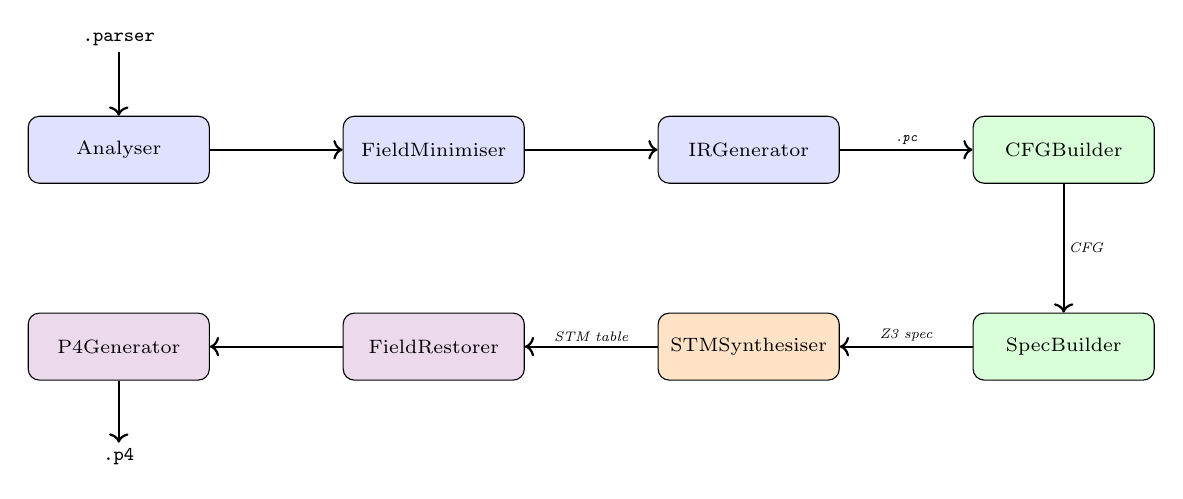
\begin{tikzpicture}[
    box/.style={draw, rectangle, rounded corners,
                minimum height=0.85cm, minimum width=2.3cm,
                font=\scriptsize, align=center},
    frontend/.style ={fill=blue!12},
    specphase/.style={fill=green!15},
    synthphase/.style={fill=orange!22},
    backend/.style  ={fill=violet!15},
    io/.style={font=\scriptsize\ttfamily, fill=white, inner sep=2pt},
    arr/.style={->, thick},
    artefact/.style={font=\tiny\itshape, fill=white, inner sep=1.5pt}
]

% Row 1
\node[box, frontend]   (a) at (0,     0)   {Analyser};
\node[box, frontend]   (b) at (4,     0)   {FieldMinimiser};
\node[box, frontend]   (c) at (8,     0)   {IRGenerator};
\node[box, specphase]  (d) at (12,    0)   {CFGBuilder};

% Row 2
\node[box, specphase]  (e) at (12,   -2.5) {SpecBuilder};
\node[box, synthphase] (f) at (8,    -2.5) {STMSynthesiser};
\node[box, backend]    (g) at (4,    -2.5) {FieldRestorer};
\node[box, backend]    (h) at (0,    -2.5) {P4Generator};

% I/O
\node[io] (in)  at (0,  1.4) {.parser};
\node[io] (out) at (0, -3.9) {.p4};

% Arrows with artefact labels
\draw[arr] (in) -- (a);
\draw[arr] (a)  -- (b);
\draw[arr] (b)  -- (c);
\draw[arr] (c)  -- (d) node[artefact, midway, above] {\texttt{.pc}};
\draw[arr] (d)  -- (e) node[artefact, midway, right] {CFG};
\draw[arr] (e)  -- (f) node[artefact, midway, above] {Z3 spec};
\draw[arr] (f)  -- (g) node[artefact, midway, above] {STM table};
\draw[arr] (g)  -- (h);
\draw[arr] (h)  -- (out);

\end{tikzpicture}%
}
\caption{The synthesis pipeline. Boxes are colour-coded by phase:
frontend (blue), specification construction (green), synthesis (orange),
and backend (violet).}
\label{fig:pipeline}

\end{figure}

We use \texttt{pycparser}~\cite{pycparser}, a Python parser for C to parse the input \texttt{.parser} program.
Since our DSL is a restricted subset of C, the AST produced by \texttt{pycparser} is a convenient starting point for the rest of the pipeline.

As shown in Figure~\ref{fig:pipeline}, the pipeline is broadly split into four stages: a frontend, a specification-construction phase, the synthesis phase, and a backend. Each stage consists of a small number of modules.

\subsection*{Frontend}

The frontend consists of the Analyser, FieldMinimiser, and IRGenerator. Together, they collect information about the program, apply field-size optimisations, and produce an IR for the next stages of the pipeline.

\begin{itemize}
    \item \textbf{Analyser:} Traverses the AST and collects information about each struct in the program, the members of \texttt{phv}
    and the fields of each member. It also records whether each field is involved in any comparison
    and the type of the comparison. This is packaged in a class we call \texttt{Info}.

    \item \textbf{FieldMinimiser:} Operates on the \texttt{Info} produced by the Analyser, applies the optimisations described in Section~\ref{sec:field-size-min} and returns an updated \texttt{Info}. This step is optional and the pipeline has been designed such that this module may be replaced to experiment with different optimisations.

    \item \textbf{IRGenerator:} Uses the updated \texttt{Info} together with another traversal over the AST to emit code in our intermediate representation, which we store in a \texttt{.pc} file.
\end{itemize}

\subsection*{Specification construction}

This stage consists of the CFGBuilder and the SpecBuilder. It also collects information which is used in optimisations during synthesis.

\begin{itemize}
    \item \textbf{CFGBuilder:} Constructs a CFG for the \texttt{.pc} IR by traversing the AST. It also rejects malformed programs. For example, those with a path that does not end in \texttt{ACCEPT} or \texttt{REJECT}.

    \item \textbf{SpecBuilder:} Walks over all possible paths in the CFG and generates a logical specification representing the parser, which is then used by the synthesiser.
\end{itemize}

\subsection*{Synthesis}

The STMSynthesiser takes the specification produced by the SpecBuilder and synthesises the FSM. It uses a CEGIS loop and constrains the search to a tabular representation of the FSM. 
This restricted format is what allows the synthesis to remain tractable.

\subsection*{Backend}

The backend consists of two modules:

\begin{itemize}
    \item \textbf{FieldRestorer:} Undoes the size and value transformations applied by the FieldMinimiser so that the synthesised FSM refers to the original fields and constants from the input.

    \item \textbf{P4Generator:} Emits the final P4 code from the synthesised FSM which is accepted as a valid parser by \texttt{p4c}.
\end{itemize}

\section{Frontend}
\label{sec:frontend}

The frontend has three modules: Analyser, FieldMinimiser, and IRGenerator. Their roles have been summarised in Section~\ref{sec:pipeline-overview}.

\subsection{Analyser}

Apart from collecting \texttt{Info}, the Analyser validates input programs to ensure that they are well-formed.
It rejects all programs that have one or more of the following bugs:
\begin{itemize}
    \item Disallowed constructs
    \item Members of \texttt{phv} that are referenced in an \texttt{Extract} call or in a condition but were not declared in the \texttt{phv} struct
    \item Header types used in the \texttt{phv} declaration that were never declared as a struct earlier
    \item Redeclaration of a struct type, or of members within a struct or within \texttt{phv}
    \item Absence of the \texttt{int parse()} function, or presence of additional functions other than \texttt{parse}.
    \item \texttt{if} conditions that do not match either the exact form (\texttt{phv.<header>.<field>~==~<constant>}) or the ternary form (\texttt{(phv.<header>.<field>~\&~<mask>)~==~<value>}).
\end{itemize}
A program that fails any of these checks raises with CompilationError.

\subsection{FieldMinimiser}
\label{sec:field-size-min}

FieldMinimiser operates on the Info produced by the Analyser and aims to reduce field sizes as much as possible while
making sure that the FSM produced by synthesis is either the same as the
one we would have got without the optimisation, or any difference should be predictable and it
can be corrected later during code generation.

The synthesis search space grows with the number of bits in each field,
and also the size of the encoded constraints. The encoding of state
transitions is linear in \texttt{max\_packet\_size}. Packet headers
typically contain wide fields that play no role in branching: for
instance, the 48-bit destination MAC in the Ethernet header is not used in
any comparison. Maintaining their full widths unnecessarily enlarges the synthesis problem.

The restrictions on the DSL make these field size minimisation optimisations easily achievable.

Every field in a header is either uncompared, compared only with exact
matches (\texttt{field == value}), or compared with at least one ternary
match. These three classes are handled separately.

\subsubsection*{Class 1: uncompared fields}

There are two sub-cases:
\begin{itemize}
    \item \textbf{The struct they belong to contains at least one compared field.} These
    uncompared fields are dropped for the sake of synthesis. The DSL
    always extracts a struct as a whole and the final P4 code also does the
    same, so these fields need not be considered in the synthesiser.

    \item \textbf{The struct they belong to contains no compared fields.} Such a struct and its fields
    cannot be dropped directly: it still has to be extracted at runtime to
    advance the packet pointer correctly and dropping it would lose the
    evidence that the extraction actually happens. Instead, we treat the whole
    struct as a single field of size 1 during synthesis. 
    a size of 0 is incorrect. An alternative approach, where such
    structs are dropped entirely for the synthesis and stitched back at
    code generation, is discussed in
    Section~\ref{sec:drop-and-stitch}.
\end{itemize}

\subsubsection*{Class 2: fields with only exact matches}

The actual values of the constants used in exact matches do not matter
for synthesis. They are just decision points. If a field is compared
against the constants $c_1, c_2, \ldots, c_n$, we can renumber them to
$0, 1, \ldots, n-1$ for synthesis and undo the renumbering at code
generation.

When branching on such a field there are at most $n+1$ outcomes:
the field equals one of the $n$ constants or it is not equal to any of them. All
values not in $\{c_1, \ldots, c_n\}$ behave the same way in the
FSM, so a single value is enough to represent them. Thus the field can be reduced to
$\lceil \log_2(n+1) \rceil+1$ bits during synthesis.

This renumbering is applied per field, which is correct because the DSL doesn't allow
multi-field conditions.

\subsubsection*{Class 3: fields with ternary matches}

Ternary matches are more difficult to handle. A single
field can satisfy a subset of the match conditions present in the program 
so the renumbering approach from Class~2 is not applicable. 


We considered two heuristics, neither of which gives a strong guarantee:
\begin{itemize}
    \item \textbf{Drop unmasked bits.} For each field, take the union of
    all bit positions that appear in any mask. Bits outside this union do
    not affect any condition, so they can all be collapsed into a single
    representative bit. This works well when masks are sparse but becomes ineffective
    when masks have many bits set.

    \item \textbf{Wildcard partitioning.} Express the field as a union of
    disjoint wildcard patterns and treat each pattern as a distinct
    symbolic constant. The number of patterns can grow quickly, so this
    does not scale.
\end{itemize}

We do not have a general bound on the reduction achieved by either heuristic.
Ternary matches are rare in practical parsing programs, so a more advanced treatment is left for future work.

\subsection{IRGenerator}

The IRGenerator emits the IR as a \texttt{.pc} file instead of directly
constructing the CFG. This is because the
specification-construction and synthesis stages of the pipeline were written
first and they used \texttt{.pc} as input and produced the FSM
output as a table. The frontend and the backend were written later. The
IRGenerator emits \texttt{.pc} to avoid making unnecessary changes in the
specification generation phase.


A \texttt{.pc} program is very similar to a \texttt{.parser} program except 
for the following changes in \texttt{.pc} programs:

\begin{itemize}
    \item There are no structs. Each field of a \texttt{phv} member
    involved in an extraction or a check is assigned a distinct variable
    name \texttt{<phv\_member>\_<field>\_<n>}, where \texttt{<n>} is a fresh
    number that keeps every name unique. This is needed to avoid two
    different fields having the same name in cases like \texttt{header1\_}'s
    field \texttt{field0} and \texttt{header1}'s field \texttt{\_field0}.
    Although such cases are rare, we preferred to have a correctness
    guarantee while renaming.

    \item The widths of the fields and the constants have been modified by the 
    FieldMinimiser.

    \item Each extract contains the size of the field being extracted along with the name

\end{itemize}

The \texttt{.pc} program corresponding to the running example
(Figure~\ref{fig:dsl-example}) is shown in Figure~\ref{fig:pc-example}.
\begin{figure}[H]
\centering
\begin{minipage}{0.6\textwidth}
\begin{lstlisting}[style=codeside, language=C]

int parse() {
    Extract(ethernet_ether_type_0,3);
    if (ethernet_ether_type_0 == 0) {
        Extract(ipv4_<first_field>_1,1);
        return ACCEPT;
    } else if (ethernet_ether_type_0 == 1) {
        Extract(arp_<first_field>_2,1);
        return REJECT;
    }
    return ACCEPT;
}
\end{lstlisting}
\end{minipage}
\caption{The \texttt{.pc} program produced by the IRGenerator for the
running example in Figure~\ref{fig:dsl-example}.}
\label{fig:pc-example}
\end{figure}

The transformations that produced this output are:
\begin{itemize}
    \item \texttt{ethernet}'s \texttt{dst} and \texttt{src} fields are
    uncompared and \texttt{ethernet} has a compared field, so they are
    dropped (Class 1a).
    \item \texttt{ether\_type} is compared against two constants
    (\texttt{0x0800} and \texttt{0x0806}), which are renumbered to
    \texttt{0} and \texttt{1}. The field is shrunk from size \texttt{16} to size \texttt{3} (Class 2).
    \item \texttt{ipv4} and \texttt{arp} have no compared fields, so both
    are shrunk to single \texttt{1} bit fields named using their
    first declared field (Class 1b).
    \item All the above fields are named using their name and the \texttt{phv} member they belong to with a globally unique
    \texttt{<n>} suffix.
\end{itemize}

A drawback of not having structs in a \texttt{.pc} program is that when a
\texttt{.parser} program has a \texttt{phv} member that has at least two
fields which are used for comparisons, the \texttt{.pc} program would have
to have separate extractions for these two fields. An idea to overcome this
is considered below.
\subsubsection*{An alternative we considered}

Instead of handling each field separately, we considered merging the
whole header into one wide field and lifting all per-field comparisons
into masked comparisons over this combined field. In principle, this could
reduce the number of states needed but this inherits the ternary handling problem 
from Class~3 and thus we did not pursue this approach.

\section{Specification Construction}
\label{sec:spec-construction}

The specification-construction stage has two modules: CFGBuilder and
SpecBuilder. Their roles have been summarised in
Section~\ref{sec:pipeline-overview}.

\subsection{CFGBuilder}

Apart from constructing the CFG, the CFGBuilder also performs
additional validation on the input. It rejects programs which have any
of the following bugs:
\begin{itemize}
    \item Programs in which the same field is extracted more than once on
    some path from the entry of \texttt{parse()} to an exit.
    \item Programs that branch on a field along some path before that
    field has been extracted on the same path.
\end{itemize}
A program that fails any of these checks raises with
\texttt{CompilationError}.

The CFG produced for the running example (Figure~\ref{fig:pc-example})
is shown in Figure~\ref{fig:cfg-example}.

\begin{figure}[H]
\centering
\resizebox{0.55\textwidth}{!}{%
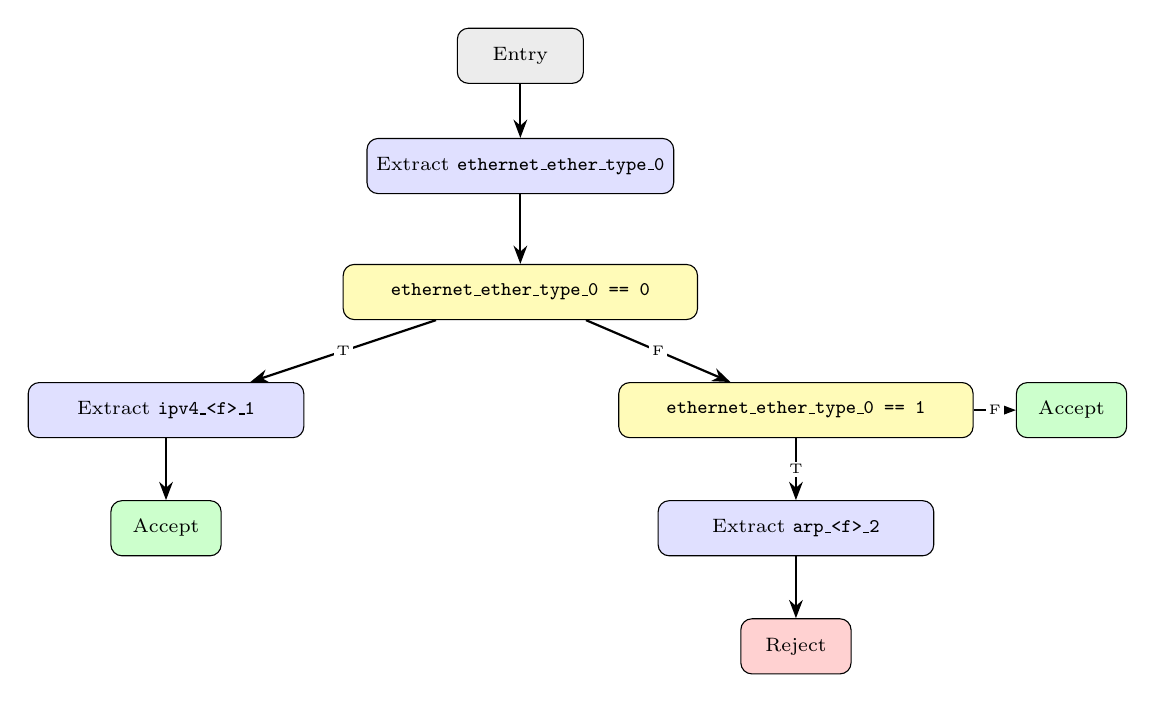
\begin{tikzpicture}[
    every node/.style={font=\scriptsize, align=center},
    entry/.style  ={draw, rectangle, rounded corners, fill=gray!15,
                    minimum height=0.7cm, minimum width=1.6cm},
    extract/.style={draw, rectangle, rounded corners, fill=blue!12,
                    minimum height=0.7cm, minimum width=3.5cm},
    decide/.style ={draw, rectangle, rounded corners, fill=yellow!28,
                    minimum height=0.7cm, minimum width=4.5cm},
    accept/.style ={draw, rectangle, rounded corners, fill=green!20,
                    minimum height=0.7cm, minimum width=1.4cm},
    reject/.style ={draw, rectangle, rounded corners, fill=red!18,
                    minimum height=0.7cm, minimum width=1.4cm},
    arr/.style={->, >=Stealth, thick},
    elabel/.style={font=\tiny, fill=white, inner sep=1pt}
]
\node[entry]   (entry) at (0,    0)    {Entry};
\node[extract] (e1)    at (0,   -1.4)  {Extract \texttt{ethernet\_ether\_type\_0}};
\node[decide]  (d1)    at (0,   -3.0)  {\texttt{ethernet\_ether\_type\_0 == 0}};
\node[extract] (e2)    at (-4.5,-4.5)  {Extract \texttt{ipv4\_<f>\_1}};
\node[accept]  (acc1)  at (-4.5,-6.0)  {Accept};
\node[decide]  (d2)    at ( 3.5,-4.5)  {\texttt{ethernet\_ether\_type\_0 == 1}};
\node[extract] (e3)    at ( 3.5,-6.0)  {Extract \texttt{arp\_<f>\_2}};
\node[reject]  (rej)   at ( 3.5,-7.5)  {Reject};
\node[accept]  (acc2)  at ( 7.0,-4.5)  {Accept};

\draw[arr] (entry) -- (e1);
\draw[arr] (e1) -- (d1);
\draw[arr] (d1) -- node[elabel] {T} (e2);
\draw[arr] (d1) -- node[elabel] {F} (d2);
\draw[arr] (e2) -- (acc1);
\draw[arr] (d2) -- node[elabel] {T} (e3);
\draw[arr] (d2) -- node[elabel] {F} (acc2);
\draw[arr] (e3) -- (rej);
\end{tikzpicture}%
}
\caption{The CFG produced by the CFGBuilder for the \texttt{.pc} program
in Figure~\ref{fig:pc-example}. Colour key: blue = \texttt{ExtractNode},
yellow = \texttt{IfThenElseNode}, green = \texttt{Accept} exit, red =
\texttt{Reject} exit.}
\label{fig:cfg-example}
\end{figure}

\subsection{SpecBuilder}

We have borrowed ideas from the implementation of
ParserHawk~\cite{parserhawk} for this module. The specification
produced is a list of expressions for the fields and a single
Boolean expression for the final accept/reject state as 
functions of the packet.

All fields are padded to \texttt{maximum\_field\_size+1} so that the
expressions for all the fields have the same Z3 bit-vector type. The
MSB is used to mark a field as ``not extracted'' on a path: the
default value of a field is a bit-vector value with MSB set and every
other bit unset. Since extracted bit-vectors have size at most
\texttt{maximum\_field\_size} and are zero-extended, no extracted
bit-vector can ever be equal to the default. This is useful in the
synthesis stage.

The specification is built using a recursive walk over the CFG,
starting at the entry node with a packet pointer(\texttt{ptr}) at the first bit
that hasn't been extracted. At every node we carry a current PHV
(\texttt{cur\_phv}). This is a list of expressions for the values of
the fields on the current path. At the entry node, every entry of
\texttt{cur\_phv} is the default value.

The specification construction happens during backtracking:

\begin{itemize}
    \item At an \texttt{ExitNode}, we return a copy of the default
    PHV along with a True/False expression based on whether the node is 
    an accept/reject node.

    \item At an \texttt{ExtractNode} for field \texttt{fno} of size
    \texttt{sz}, we set
\begin{lstlisting}[style=codeside, language=C]
cur_phv[fno] = ZeroExt(maximum_field_size+1-sz, Extract(ptr+sz-1, ptr, packet))
\end{lstlisting}
    and recurse on the next node with the packet pointer advanced by
    \texttt{sz}. When the recursion returns, we overwrite the field's
    entry in the returned PHV with the same expression, since the
    \texttt{ExitNode}s at the leaves return only the default values.
    It can be observed that no overwrite happens here, since no field
    is extracted twice on any path.

    \item At an \texttt{IfThenElseNode} branching on field
    \texttt{fno} with value \texttt{v}, we walk the true and false
    branches to obtain \texttt{(true\_phv, true\_state)} and
    \texttt{(false\_phv, false\_state)}. For every field $i$, the
    $i$-th entry of the merged PHV is \texttt{If(cur\_phv[fno] == v,
    true\_phv[i], false\_phv[i])} (or with a mask, for ternary
    matches). The accept/reject state is merged similarly.
\end{itemize}

The expressions returned at the root are the specification given to
the synthesiser. For the running example
(Figure~\ref{fig:cfg-example}), the specification is:

\begin{lstlisting}[style=codeside, language=C]
ether_type = ZeroExt(1, Extract(2, 0, packet))
ipv4       = If(ZeroExt(1, Extract(2, 0, packet)) == 0,
                ZeroExt(3, Extract(3, 3, packet)),
                default)
arp        = If(ZeroExt(1, Extract(2, 0, packet)) == 0,
                default,
                If(ZeroExt(1, Extract(2, 0, packet)) == 1,
                   ZeroExt(3, Extract(3, 3, packet)),
                   default))
state      = If(ZeroExt(1, Extract(2, 0, packet)) == 0,
                True,
                If(ZeroExt(1, Extract(2, 0, packet)) == 1,
                   False,
                   True))
\end{lstlisting}

where \texttt{default} is the bit-vector \texttt{1000} in binary.
The largest field after minimisation is of size 3, so
\texttt{maximum\_field\_size+1} = 4 bits.


\section{Synthesis}
\label{sec:synthesis}

This is where the logical formula constructed in the previous phase
is used to run a CEGIS loop and synthesise the FSM as a
table.

The design of the FSM is inspired by the P4 parser state
machine described in Figure~\ref{fig:c-vs-p4}. We considered two
designs that differ in a small way. We describe the first design in
detail in this section and briefly mention how the second design is 
different.

\subsection{First Design}

This design works only for programs with exact comparisons and is less general than the 
second design, but we describe it in detail because it
motivates the second design and also enables the drop-and-stitch
optimisation discussed in Section~\ref{sec:drop-and-stitch}.

The FSM is expressed as a table. Each state has a default
field which it extracts and branches on, and a default next state
which is taken when none of the listed transitions are satisfied.
Apart from this, there is a list of transition entries, each of the
form \texttt{(current\_state, match\_value, next\_state)}.

When making a state transition, the field extracted in that
state is compared against all the transition entries for that state. 
The matching entry is used to perform the transition. Since only
exact comparisons are involved, at most one entry can match and if none of them
matches the default transition is taken.

The synthesis itself is a CEGIS loop with two components: a
Generator and a Verifier. The Generator produces FSMs compliant with the
counterexamples seen so far. 
The Verifier checks if it satisfies the specification for
every possible input packet by trying to find a counterexample. 
Each counterexample is added as a fresh correctness
constraint to the Generator and the loop continues 
until the Verifier finds no
counterexample for the synthesised FSM or until the Generator cannot synthesise 
an FSM satisfying the constraints. 
The two have similar designs, so we describe the
Generator only. We run a fresh CEGIS loop for each candidate
\texttt{(table\_size, no\_states)} pair and take the first state
machine the Verifier accepts as the output.

\subsubsection*{Generator}

The Generator enforces three kinds of basic constraints on the state-machine
table:

\begin{itemize}
    \item \textbf{Domain constraints.} For example, the default field
    number of every state must be one of the allowed field numbers.

    \item \textbf{Determinism constraints.} No two transition entries
    from the same state may have the same matched value but different
    next states.

    \item \textbf{Ordering for optimisation.} A state transition can
    only go from a state with a lower number to a state with a higher
    number.
\end{itemize}

In addition to these structural constraints, the Generator encodes
the symbolic simulation of the FSM and the per-packet
correctness constraints.

We simulate the FSM by repeatedly applying the transition,
starting from \texttt{cur\_state = 0},
\texttt{cur\_packet\_ptr = 0}, and \texttt{cur\_phv} set to the
default values. The ordering constraint above forces the synthesised
FSM to be loopless. We accept this restriction since
the input programs are loopless as well. In such a FSM applying transitions
for \texttt{no\_states} steps is enough to reach accept or reject.

A transition takes
\texttt{(cur\_phv, cur\_state, cur\_packet\_ptr)} to
\texttt{(next\_phv, next\_state, next\_packet\_ptr)} parameterised
by the table variables. All three components are nested \texttt{If} expressions.
\texttt{cur\_state} is integer-valued (the current state number),
\texttt{cur\_phv} is a list of bit-vector expressions for the fields and
\texttt{cur\_packet\_ptr} is an integer expression giving the bit
position of the next field to be extracted.

The transition is itself one nested \texttt{If} expression. It is
built in four steps: field extraction, default transition,
match lookup, and bounds check. These are executed in that order.
Each step overrides the previous when its condition holds. 
Below, \texttt{sz} stands for \texttt{field\_sizes[f]} and \texttt{M} for
the padded width \texttt{maximum\_field\_size + 1}.

\textbf{1. Field extraction.} For every \texttt{(s, f, p)} with
\texttt{p + sz $\le$ max\_packet\_size}:
\begin{lstlisting}[style=codeside, language=C]
g = (cur_state == s) and (default_field[s] == f)
                     and (cur_packet_ptr == p)
next_packet_ptr = If(g, p + sz, next_packet_ptr)
next_phv[f]     = If(g, ZeroExt(M - sz,
                                Extract(p + sz - 1, p, packet)),
                        next_phv[f])
\end{lstlisting}

\textbf{2. Default transition.} \texttt{next\_state} is initialised
to \texttt{cur\_state}, so accept and reject states don't transition.
For every state \texttt{s}:
\begin{lstlisting}[style=codeside, language=C]
next_state = If(cur_state == s,
                default_next_state[s],
                next_state)
\end{lstlisting}

\textbf{3. Match lookup.} For every \texttt{(idx, s, f)}:
\begin{lstlisting}[style=codeside, language=C]
g = (cur_state == s) and (default_field[s] == f)
                     and (entry_state[idx] == s)
                     and (next_phv[f] == entry_match_value[idx])
next_state = If(g, entry_next_state[idx], next_state)
\end{lstlisting}

\textbf{4. Bounds check.} For every \texttt{(s, f, p)} with
\texttt{p + sz > max\_packet\_size}:
\begin{lstlisting}[style=codeside, language=C]
g = (cur_state == s) and (default_field[s] == f)
                     and (cur_packet_ptr == p)
next_state = If(g, reject, next_state)
\end{lstlisting}

For each input packet (a bit-vector constant) added during the CEGIS
loop, the correctness constraint checks whether the final state and PHV match
the specification after \texttt{no\_states} simulation steps.

To illustrate, the synthesised FSM for the running
example's \texttt{.pc} program (Figure~\ref{fig:pc-example}) is
shown in Figure~\ref{fig:running-stm-fd}. Three states and two
table entries suffice.

\begin{figure}[H]
\centering
\begin{minipage}{0.62\textwidth}
\centering
\footnotesize
\begin{tabular}{c l c c}
\hline
State & Default field & Entries (val $\to$ next) & Default next \\
\hline
0 & \texttt{ethernet\_ether\_type\_0} & $0 \to 1$, $1 \to 2$ & accept \\
1 & \texttt{ipv4\_<f>\_1}             &                       & accept \\
2 & \texttt{arp\_<f>\_2}              &                       & reject \\
\hline
\end{tabular}
\end{minipage}
\hfill
\begin{minipage}{0.32\textwidth}
\centering
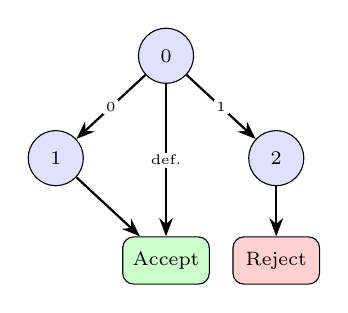
\begin{tikzpicture}[
    every node/.style={font=\scriptsize, align=center},
    state/.style ={draw, circle, fill=blue!12, minimum size=0.7cm},
    accept/.style ={draw, rectangle, rounded corners, fill=green!20,
                    minimum height=0.6cm, minimum width=1.1cm},
    reject/.style ={draw, rectangle, rounded corners, fill=red!18,
                    minimum height=0.6cm, minimum width=1.1cm},
    arr/.style={->, >=Stealth, thick},
    elabel/.style={font=\tiny, fill=white, inner sep=1pt}
]
\node[state]  (s0)  at ( 0,    0)   {0};
\node[state]  (s1)  at (-1.4, -1.3) {1};
\node[state]  (s2)  at ( 1.4, -1.3) {2};
\node[accept] (acc) at ( 0,   -2.6) {Accept};
\node[reject] (rej) at ( 1.4, -2.6) {Reject};

\draw[arr] (s0) -- node[elabel] {0}    (s1);
\draw[arr] (s0) -- node[elabel] {1}    (s2);
\draw[arr] (s0) -- node[elabel] {def.} (acc);
\draw[arr] (s1) -- (acc);
\draw[arr] (s2) -- (rej);
\end{tikzpicture}
\end{minipage}
\caption{The synthesised FSM for the running example's
\texttt{.pc} program for the first design. Left: the state-table
representation. Right: the corresponding state-transition graph.
State numbers in the graph match the rows of the table.}
\label{fig:running-stm-fd}
\end{figure}

\subsubsection*{Limitations of the first design}

\textbf{State replication.} Since each field can be extracted only
once on a path and must be branched on immediately, we end up
replicating states unnecessarily. Consider:

\begin{lstlisting}[style=codeside, language=C]
Extract(field0, 4);
Extract(field1, 1);
if (field0 == 4) {
    ...
} else {
    ...
}
\end{lstlisting}

The state extracting \texttt{field1} has to be replicated, since the
branch on \texttt{field0} has to happen first.

\textbf{Priority among transitions (with ternary matches).} We also
tried to extend the first design to support ternary comparisons by
adding a mask alongside the value in each transition entry. Exact
comparisons would use a mask of size
\texttt{maximum\_field\_size} with all bits set. 
This extension runs into a problem when the values matched by two ternary conditions overlap.
Consider:

\begin{lstlisting}[style=codeside, language=C]
Extract(field0, 4);
if ((field0 & 3) == 1) {
    if ((field0 & 12) == 4) {
        ...
    }
    ...
}
...
\end{lstlisting}

The state extracting \texttt{field0} needs both a transition for the
case where both masks are satisfied and a transition for the case
where only the outer mask is satisfied. These cannot be encoded as
transitions from a single state without enforcing a priority between
them. The priority could be expressed naturally (transitions checked
first having higher priority), but we did not pursue this. A
FSM with priority-ordered transitions is not standard, and
a parser is typically expected to have at most one matching
transition at every state.

\subsection{Second Design}

We observed that the issues in the previous design came from
allowing only the state which extracted a field to branch on it. In
this design we relax this constraint. Every state must have a
default field assigned to it like in the previous design and it may
or may not extract it. It may or may not branch on it as well.
This corresponds to the case where there is only a default
transition.

Some small changes need to be made in the transitions. We now need
to ensure two things: one is that while branching on a field, we
do so only if it has been extracted, and the other is that while
extracting, we do so only if it hasn't been extracted before.

The first is ensured in the match-lookup step of the transition. A
table entry for a state is considered only if the default field's
expression for that state is not equal to its default value, which
can happen only if the field has been extracted on this path. If it
is equal to the default, the transition based on it is not made and
the entry is not used.

The second is ensured by checking, during an extract, that the field
expression equals the default value. This can happen only when it
has not been extracted before. The bounds-check step also performs
a similar check so that a transition to reject is taken only when the state
actually attempts an extraction.

The fact that the default value can never be taken by an extracted
field (ensured during specification construction) is what makes
these checks possible.

Since we iterate over the number of table entries and the number of
states, we will not encounter table entries that don't make sense.
If there is no table entry for a state, the default transition is
taken for every value of the field. 
We would also have to run an additional graph traversal algorithm to find the state 
which extracts the field after the synthesis as the FSM itself doesn't 
explicitly mention whether a particular state performs an extraction or not.  

It can be seen that both of the problems of the original state
machine are solved by this design. But it makes applying certain
optimisations harder due to the extra flexibility.

\subsubsection*{Constant synthesis}

If there are only exact matches in a program, we can collect the
constants and constrain the values that the \texttt{match\_value}s
in the table can take, to reduce the search space. This can be done
for ternary matches as well if we are following the second design.
Both \texttt{match\_value}s and \texttt{match\_mask}s can be
constrained to the constants and masks appearing in the program.

\subsubsection*{An observation on iteration speed}

Running the synthesis from a smaller number of states and table
entries to larger ones works faster than directly instantiating the
larger problems, even when a new Z3 solver is created for each
iteration. This is probably because of the CDCL(T) algorithm that Z3
runs. It caches some clauses in its memory across calls within
the same process, which results in the speedup.

This is one of the reasons why we kept the iteration over table
entries and states. The other is that it leads to a simpler
transition encoding, without having to worry about inconsistent
entries in the tables.


\section{Backend}
\label{sec:backend}

The backend has two modules, FieldRestorer and P4Generator, whose
roles have been summarised in Section~\ref{sec:pipeline-overview}.

\subsection{FieldRestorer}

The FieldRestorer reverses the transformations done by the
FieldMinimiser. The \texttt{Info} class produced by the frontend
contains all the information needed for this. It remembers the
original bit-widths of the fields and the original
constants. The FieldRestorer reads from \texttt{Info} and maps
every entry of the synthesised state-machine table back to its
original form.

\subsection{P4Generator}

The P4Generator walks the restored FSM and emits the
final P4 code. P4 allows only the extraction of whole headers, not
field by field. The synthesised FSM extracts one field
per state, so the P4Generator groups the per-field extracts of the
same header into a single \texttt{packet.extract(hd.<header>)}
call. This is done by a simple graph traversal that identifies,
for each header, the state that extracts its first field. That
state then emits the whole-header extract in the P4 output.

This grouping is especially important for the second design as there may be fields which 
perform no extractions.

\subsection{Drop-and-stitch optimisation}
\label{sec:drop-and-stitch}

We discussed in Section~\ref{sec:field-size-min} that headers
which have none of their fields used in any comparison may be
dropped completely from the synthesis and stitched back into the
FSM afterwards. This is the optimisation referred to
there. We believe it is easiest to apply with the first design.

Realistic parsers tend to stop branching after extracting transport
protocol headers, and all of the branching conditions are mostly exact matches.
In such parsers, most of the headers are uncompared. Dropping them
from the input before synthesis reduces the number of states the
synthesiser has to deal with significantly.

Consider the parse function:

\begin{lstlisting}[style=codeside, language=C]
int parse() {
    Extract(phv.hdr0);
    Extract(phv.hdr1);
    Extract(phv.hdr2);
    if (phv.hdr0.field0 == 3) {
        if (phv.hdr1.field1 == 2) {
            Extract(phv.hdr4);
        }
    } else if (phv.hdr0.field0 == 4) {
        if (phv.hdr1.field1 == 5) {
            Extract(phv.hdr5);
        }
    }
    return ACCEPT;
}
\end{lstlisting}

where \texttt{hdr0.field0} and \texttt{hdr1.field1} are the only
compared fields, and \texttt{hdr2}, \texttt{hdr4} and \texttt{hdr5}
are uncompared. We
drop \texttt{hdr2}, \texttt{hdr4} and \texttt{hdr5} from the input
and run synthesis on the remainder. After this drop, all paths
through the program reach Accept with the same observable
behaviour, so the synthesiser produces the straight-line state
machine in Figure~\ref{fig:dropped-stm}.

\begin{figure}[H]
\centering
\resizebox{0.6\textwidth}{!}{%
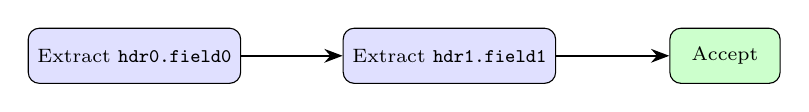
\begin{tikzpicture}[
    every node/.style={font=\scriptsize, align=center},
    extract/.style={draw, rectangle, rounded corners, fill=blue!12,
                    minimum height=0.7cm, minimum width=2.5cm},
    accept/.style ={draw, rectangle, rounded corners, fill=green!20,
                    minimum height=0.7cm, minimum width=1.4cm},
    arr/.style={->, >=Stealth, thick}
]
\node[extract] (s0)  at (0,0)   {Extract \texttt{hdr0.field0}};
\node[extract] (s1)  at (4,0)   {Extract \texttt{hdr1.field1}};
\node[accept]  (acc) at (7.5,0) {Accept};
\draw[arr] (s0) -- (s1);
\draw[arr] (s1) -- (acc);
\end{tikzpicture}%
}
\caption{The synthesised FSM after dropping
\texttt{hdr2}, \texttt{hdr4} and \texttt{hdr5} from the input.}
\label{fig:dropped-stm}
\end{figure}

We now stitch the dropped headers back into this machine and add
the missing transitions. From the CFG, different values of
\texttt{hdr0.field0} lead to different sequences of further
extractions, so the single outgoing transition out of the state
extracting \texttt{hdr0.field0} is split into three: one each for
\texttt{== 3}, \texttt{== 4} and default. The state extracting
\texttt{hdr1.field1} is replicated across all three branches, since
\texttt{hdr1} is extracted on every path through the original
program. The \texttt{== 3} and \texttt{== 4} replicas branch
further on \texttt{hdr1.field1} (going on to extract \texttt{hdr4}
on one and \texttt{hdr5} on the other), while the default replica
does not branch. \texttt{hdr2} appears in multiple places in the
stitched machine for similar reasons. The final FSM is
shown in Figure~\ref{fig:stitched-stm}.

\begin{figure}[H]
\centering
\resizebox{0.6\textwidth}{!}{%
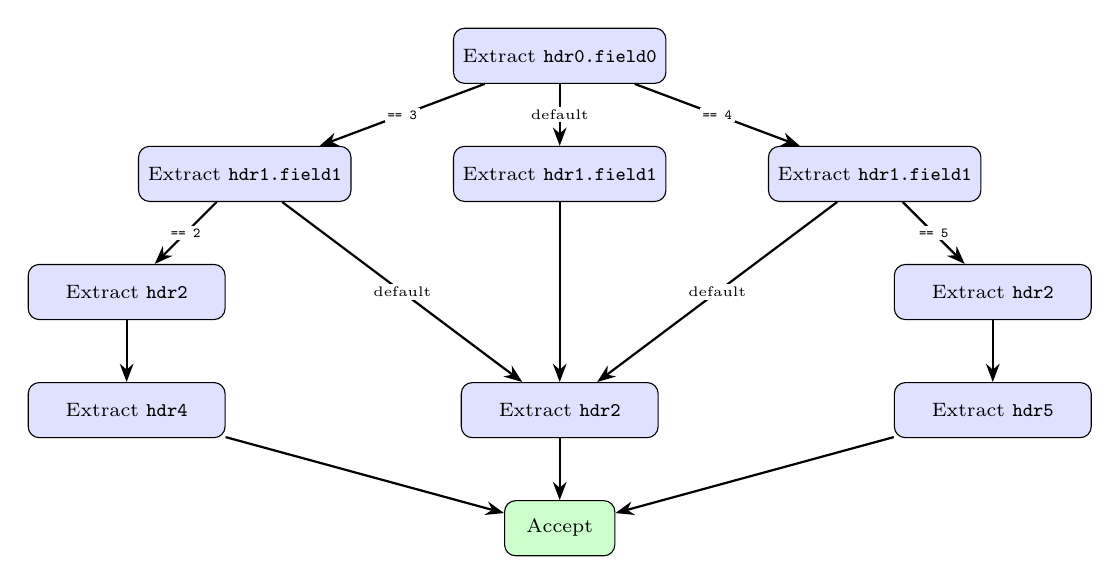
\begin{tikzpicture}[
    every node/.style={font=\scriptsize, align=center},
    extract/.style={draw, rectangle, rounded corners, fill=blue!12,
                    minimum height=0.7cm, minimum width=2.5cm},
    accept/.style ={draw, rectangle, rounded corners, fill=green!20,
                    minimum height=0.7cm, minimum width=1.4cm},
    arr/.style={->, >=Stealth, thick},
    elabel/.style={font=\tiny, fill=white, inner sep=1pt}
]
\node[extract] (s0)   at ( 0,    0)   {Extract \texttt{hdr0.field0}};
\node[extract] (s1a)  at (-4,   -1.5) {Extract \texttt{hdr1.field1}};
\node[extract] (s1c)  at ( 0,   -1.5) {Extract \texttt{hdr1.field1}};
\node[extract] (s1b)  at ( 4,   -1.5) {Extract \texttt{hdr1.field1}};
\node[extract] (s2_4) at (-5.5, -3)   {Extract \texttt{hdr2}};
\node[extract] (s2_5) at ( 5.5, -3)   {Extract \texttt{hdr2}};
\node[extract] (sh4)  at (-5.5, -4.5) {Extract \texttt{hdr4}};
\node[extract] (sh5)  at ( 5.5, -4.5) {Extract \texttt{hdr5}};
\node[extract] (s2d)  at ( 0,   -4.5) {Extract \texttt{hdr2}};
\node[accept]  (acc)  at ( 0,   -6)   {Accept};

\draw[arr] (s0)  -- node[elabel] {\texttt{== 3}}  (s1a);
\draw[arr] (s0)  -- node[elabel] {\texttt{== 4}}  (s1b);
\draw[arr] (s0)  -- node[elabel] {default}        (s1c);
\draw[arr] (s1a) -- node[elabel] {\texttt{== 2}}  (s2_4);
\draw[arr] (s1a) -- node[elabel] {default}        (s2d);
\draw[arr] (s1b) -- node[elabel] {\texttt{== 5}}  (s2_5);
\draw[arr] (s1b) -- node[elabel] {default}        (s2d);
\draw[arr] (s1c) -- (s2d);
\draw[arr] (s2_4) -- (sh4);
\draw[arr] (s2_5) -- (sh5);
\draw[arr] (s2d)  -- (acc);
\draw[arr] (sh4)  -- (acc);
\draw[arr] (sh5)  -- (acc);
\end{tikzpicture}%
}
\caption{The FSM after stitching back \texttt{hdr2},
\texttt{hdr4} and \texttt{hdr5}. The state extracting \texttt{hdr2}
on the default paths is shared.}
\label{fig:stitched-stm}
\end{figure}

This stitched FSM is equivalent to what the synthesiser
would have produced if the uncompared headers had been kept, but
is obtained much faster. We believe that the stitching procedure
can be fully automated. It would be a useful extension to make the
pipeline practical on larger parsers, where the synthesis problem
with all fields kept becomes intractable.


\chapter{Testing and Evaluation}
\label{ch:testing-evaluation}

We tested the design by running each configuration on a set of
hand-written parsers and reviewing the synthesised state machine for
correctness. A small Python helper renders the synthesised state
machine as a PDF, which made the manual review easier.

We evaluate the design separately for input programs that use only
exact comparisons and for programs that involve ternary
comparisons since the supported configurations differ in the two
cases. 

\section{Exact comparisons}
\label{sec:eval-exact}

We ran four benchmarks with each of the following configurations
for both Design~1 and Design~2. \texttt{max\_states} and
\texttt{max\_table\_entries} were both set to ten, and a timeout of
20 minutes was imposed on each run.

\begin{enumerate}
    \item Constant synthesis and field minimisation.
    \item Field minimisation only.
    \item Constant synthesis only.
    \item No optimisation.
\end{enumerate}

Table~\ref{tab:eval-exact-fieldsizes} reports the maximum bit width
of a packet with and without field minimisation on these benchmarks.
Table~\ref{tab:exact-results} reports the resulting state count,
table-entry count and synthesis time for each configuration for
both designs.

\begin{table}[H]
\centering
\rowcolors{2}{blue!5}{white}
\begin{tabular}{lcc}
\hline
\rowcolor{blue!20}
\textbf{Benchmark} & \textbf{field min.\ on (bits)} & \textbf{field min.\ off (bits)} \\
\hline
\texttt{linear}                & 3 & 72  \\
\texttt{single\_if}            & 4 & 56  \\
\texttt{multiple\_if}          & 7 & 88  \\
\texttt{check\_after\_extract} & 5 & 72  \\
\hline
\end{tabular}
\caption{Maximum bit width of a packet with and without
field minimisation, on the exact-comparison benchmarks.}
\label{tab:eval-exact-fieldsizes}
\end{table}

\begin{table}[H]
\centering
\resizebox{\textwidth}{!}{%
\begin{tabular}{l|cc|ccc|ccc}
\hline
\rowcolor{blue!20}
\textbf{Benchmark} & \textbf{CS} & \textbf{FM}
& \multicolumn{3}{c|}{\textbf{Design 1}}
& \multicolumn{3}{c}{\textbf{Design 2}} \\
\rowcolor{blue!20}
 & & & \textbf{States} & \textbf{Entries} & \textbf{Time (s)}
     & \textbf{States} & \textbf{Entries} & \textbf{Time (s)} \\
\hline
\texttt{linear}                 & on  & off & 3 & 0 & 1.23   & 3 & 0 & 2.44    \\
\texttt{linear}                 & on  & on  & 3 & 0 & 0.43   & 3 & 0 & 0.24    \\
\texttt{linear}                 & off & off & 3 & 0 & 1.44   & 3 & 0 & 1.84    \\
\texttt{linear}                 & off & on  & 3 & 0 & 0.45   & 3 & 0 & 0.19    \\
\hline
\texttt{single\_if}             & on  & off & 3 & 1 & 68.08  & 3 & 1 & 51.89   \\
\texttt{single\_if}             & on  & on  & 3 & 1 & 14.86  & 3 & 1 & 21.98   \\
\texttt{single\_if}             & off & off & 3 & 1 & 55.11  & 3 & 1 & 50.49   \\
\texttt{single\_if}             & off & on  & 3 & 1 & 11.18  & 3 & 1 & 23.41   \\
\hline
\texttt{check\_after\_extract} & on  & off & 4 & 2 & 132.97 & 4 & 2 & 164.23  \\
\texttt{check\_after\_extract} & on  & on  & 4 & 2 & 35.47  & 4 & 2 & 144.92  \\
\texttt{check\_after\_extract} & off & off & 4 & 2 & 159.22 & 4 & 2 & 279.61  \\
\texttt{check\_after\_extract} & off & on  & 4 & 2 & 39.28  & 4 & 2 & 133.84  \\
\hline
\texttt{multiple\_if}           & on  & off & 7 & 3 & 931.27 & 6 & 2 & 557.88  \\
\texttt{multiple\_if}           & on  & on  & 7 & 3 & 339.76 & 6 & 2 & 249.91  \\
\texttt{multiple\_if}           & off & off & 7 & 3 & 696.18 & 6 & 2 & 652.19  \\
\texttt{multiple\_if}           & off & on  & 7 & 3 & 421.73 & 6 & 2 & 330.57  \\
\hline
\end{tabular}%
}
\caption{Synthesis results on the exact-comparison benchmarks
across all four \textsf{CS}/\textsf{FM} configurations, for both
designs. \textsf{CS} stands for constant synthesis and \textsf{FM}
for field minimisation.}
\label{tab:exact-results}
\end{table}

Field minimisation was the most effective optimisation. It produced
a 3--5$\times$ speedup over the unminimised baseline on most
benchmarks. Constant synthesis produced a reasonable speedup on
some benchmarks but performed worse on others. On
\texttt{multiple\_if}, the second design produced an FSM with one
fewer state and one fewer table entry than the first
and was faster. On the other benchmarks, where both
designs produced state machines of the same size, the first design
ran faster due to its smaller constraints.

We additionally evaluated the best-performing configuration on
realistic parsers translated from the ParserHawk benchmarks, with
a timeout of 30 minutes, a maximum of 10 states and a maximum of
10 table entries. Synthesis did not complete within the allotted
time. This indicates that more efficient optimisation techniques
are required to make the approach practically applicable, and is
an important direction for future work.

\clearpage
\section{Ternary comparisons}
\label{sec:eval-ternary}

Only Design~2 supports ternary comparisons, as discussed in
Section~\ref{sec:synthesis}, so we evaluated it with two
configurations: field minimisation on, and field minimisation off.
Field minimisation was applied only on the fields that participate
in exact comparisons or in no comparison at all. Fields involved in
ternary comparisons were left untouched.

A timeout of 20 minutes was imposed on each run. The benchmarks
were run with eight states and eight table entries as the maximum.
Table~\ref{tab:eval-ternary-fieldsizes} reports the maximum bit width of a packet.
Table~\ref{tab:eval-ternary} reports the resulting state count,
table-entry count and synthesis time. A dash indicates that the
configuration timed out.

\begin{table}[H]
\centering
\rowcolors{2}{blue!5}{white}
\begin{tabular}{lcc}
\hline
\rowcolor{blue!20}
\textbf{Benchmark} & \textbf{field min.\ on (bits)} & \textbf{field min.\ off (bits)} \\
\hline
\texttt{single\_if\_else}      & 6  & 12  \\
\texttt{multiple\_if}          & 9  & 36  \\
\texttt{check\_after\_extract} & 10 & 72  \\
\texttt{nested\_if\_else2}     & 6  & 12  \\
\texttt{nested\_if\_else1}     & 12 & 104 \\
\hline
\end{tabular}
\caption{Maximum bit width of a packet with and without
field minimisation, on the ternary benchmarks.}
\label{tab:eval-ternary-fieldsizes}
\end{table}

\begin{table}[H]
\centering
\rowcolors{2}{blue!5}{white}
\begin{tabular}{lcccc}
\hline
\rowcolor{blue!20}
\textbf{Benchmark} & \textbf{Field min.} & \textbf{States} & \textbf{Entries} & \textbf{Time (s)} \\
\hline
\texttt{single\_if\_else}      & on  & 4 & 1 & 18.85   \\
\texttt{single\_if\_else}      & off & 4 & 1 & 18.55   \\
\texttt{multiple\_if}          & on  & 4 & 3 & 432.67  \\
\texttt{multiple\_if}          & off & 4 & 3 & 484.76  \\
\texttt{check\_after\_extract} & on  & 4 & 2 & 79.64   \\
\texttt{check\_after\_extract} & off & 4 & 2 & 206.32  \\
\texttt{nested\_if\_else2}     & on  & 4 & 2 & 56.29   \\
\texttt{nested\_if\_else2}     & off & 4 & 2 & 64.38   \\
\texttt{nested\_if\_else1}     & on  & 6 & 3 & 602.07  \\
\texttt{nested\_if\_else1}     & off & - & - & timeout \\
\hline
\end{tabular}
\caption{Synthesis results on ternary benchmarks with Design~2.
Field minimisation was applied only on fields that do not
participate in ternary comparisons.}
\label{tab:eval-ternary}
\end{table}

The state and table-entry counts match across the two
configurations for every benchmark that completed and the run with 
field minimisation on runs faster always.
The speedup from field minimisation is substantial
on \texttt{check\_after\_extract} and \texttt{nested\_if\_else1}.
On \texttt{nested\_if\_else1} the minimised configuration completes
in about ten minutes while the unminimised one times out.


\chapter{Conclusion and Future Work}
\label{ch:conclusion}

We have thus built a pipeline which takes a C-like sequential packet
parsing code and produces a state machine as a P4 parser using program
synthesis. The source code is available at~\cite{parsercompiler26_repo}.

\section{Limitations}
\label{sec:limitations}

Our design has a few limitations:
\begin{enumerate}
    \item The DSL is very restrictive. It only allows extracts,
    no lookaheads, no conditions involving \texttt{\&\&} or
    \texttt{||}, and no cross-packet state. All of these would be
    desirable in some cases for packet processing.

    \item We have ignored the difference between the byte order in
    network packets and the way structs are stored in memory.

    \item Bitmask handling doesn't scale well. See the Class~3 case
    in Section~\ref{sec:field-size-min} and the ``alternative we
    considered'' subsection in the IRGenerator.

    \item The state machine produced doesn't necessarily have the
    minimum number of states.
\end{enumerate}

\section{Future Work}

To build on this work:
\begin{enumerate}
    \item Extend the design to overcome the limitations above.

    \item Develop a more efficient method to handle bitmasks and automate the drop-and-stitch optimisation.
    
    \item Investigate better synthesis analyses to improve
    performance and scalability.

    \item Use these ideas for further analyses to enable vector
    processing, in particular handling the control flow divergence
    that arises due to parsing.
\end{enumerate}

% --- References ---
\bibliographystyle{plain}
\bibliography{references}

\chapter*{Acknowledgement of LLM Usage}
LLMs were helpful in the final stages of this project. They were
used in the following ways.

\begin{enumerate}
    \item Formatting the report in LaTeX and producing the diagrams
    and tables in it.
    \item Rapid prototyping of ideas added in the final stage,
    mainly to check the applicability of the FieldRestorer
    optimisations. The LLM was not able to produce a working
    implementation of the optimisation, and that code has not been
    added to the GitHub repository.
    \item Writing PowerShell scripts to run the benchmarks.
    \item Writing a few small functions in the final design that
    involved Python features I was not familiar with, such
    as the \texttt{re} module and some additional file-handling
    operations.
    \item Generating the boilerplate code that follows the
    synthesised parser in the P4 output, such as the ingress and
    egress processing blocks.
\end{enumerate}
\end{document}
